\scanpage{56}

Bruxelles 5, le 15 décembre 1966\\

Cher Grothendieck,\\

Je lis aujourd'hui ta lettre du 28 - Après avoir tourné 7 fois ma langue dans ma bouche, je réjète mon objection à l'hypothèse ``tout quotient de tout sous-module de $M$ est separé pour la topologie $J$-adique'', qui \uline{n'est pas}\inserted{ en général} vérifiée pour $M$ de type fini sur \deleted{\unsure{B}}la $A$-algèbre $B$, $A$ et $B$ noethériens, $JB\subset R(B)$.

\[
\begin{aligned}
&\text{\uline{Contre exemple} :}\quad A\ \text{noethérien local},\quad J=m\\
&\hphantom{\text{Contre exemple :}\quad} B=A[[T]],\quad M=B
\end{aligned}
\]

comme \uline{$A$-module}, $B\sim A_s^N$, donc tout module quotient de $A_s^{(N)}$ est quotient d'un sous-$A$-module de $B$. \deleted{\unsure{$T$|7|Un}} Un module ayant un système dénombrable de générateurs n'a aucune raison d'être séparé !

Bien sûr, les démonstrations \deleted{ne} n'utilisent que des quotient et sous-modules comme $B$-modules.

J'essayerai encore une fois de lire 19.7.

Bien à toi\\

P. Deligne\\

P.S. Je rappelle que l'adresse où tu me touches le plus rapidement est :

S.M.\quad P. Deligne\\
Athénée Royal de Rösrath\\
BPS 8\\
FBA - (forces belges en Allemagne)\\

P.S. Je commence à lire $\overline{\underline{\mathrm{IV}}}$ \S\,16. La démonstration de 16.1.5 est canulée, comme on le voit en prenant $X=\operatorname{Spec}(k[T])$, $Y=\operatorname{Spec}(k[T])\amalg\operatorname{Spec}(k)$, tous deux affins.

\diagram{\begin{tikzcd}[ampersand replacement=\&,row sep=2pt,column sep=2pt]
Y\arrow[d,xshift=-9pt] \& \left\{\ 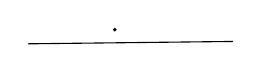
\begin{tikzpicture}[baseline=0pt]\draw (0,0)--(2.6,0.03);\fill (1.1,.18) circle (.025);\end{tikzpicture}\right.\\
X \& \left\{\ 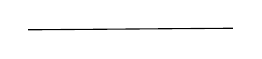
\begin{tikzpicture}[baseline=0pt]\draw (0,0)--(2.6,.02);\end{tikzpicture}\right.
\end{tikzcd}}

Avec les notations de 16.1.15 (\unsure{1|i}), $J=0$, mais les voisinages infinitésimaux de $Y$ ne sont pas \deleted{\unsure{nuls en $\operatorname{Spec}(k)$}} triviaux en $\operatorname{Spec}(k)$

J'ignore si la proposition est vraie -
% archive sheet number: 55
